\subsubsection{Scenario S2: L'organizzatore seriale}

Lo Scenario S2 ha richiesto agli utenti di simulare l'organizzazione del materiale didattico all'inizio di un nuovo anno accademico. L'obiettivo operativo consisteva nel creare una gerarchia di file configurando una cartella dedicata all'esame di "Basi di Dati" , procedendo poi al caricamento del programma ufficiale del corso al suo interno. Infine, l'utente doveva caricare un file audio della lezione e convertirlo in testo, sfruttando gli strumenti di Intelligenza Artificiale messi a disposizione dalla piattaforma.

\paragraph{Analisi delle prestazioni generali}

La totalità dei partecipanti ha completato con successo lo Scenario S2 in entrambe le configurazioni del sistema (Tabella~\ref{tab:6-s2-1}). L'efficacia della riprogettazione si manifesta in modo marcato attraverso un abbattimento drastico dei tre indicatori prestazionali principali, tutti confermati da forti riscontri sul piano statistico. In primo luogo, la media degli errori registra una contrazione del 83,33\%, scendendo da 2,80 nella versione originale ad appena 0,47 nella versione B. Parallelamente, si assiste a un progresso netto e confermato sul piano statistico per il tempo medio di esecuzione, ridotto del 39,72\% (da 4.37.16 a 2.47.08), e per il numero medio di click richiesti per portare a termine il flusso di lavoro, calati del 59,55\% (da 50,60 a 20,47). A riprova di questi risultati, la difficoltà percepita espressa tramite la mediana evidenzia un decremento, scendendo da un valore pari a 3 (neutro) a 2 (facile). Questa tendenza positiva è supportata anche dalle medie riportate in Figura~\ref{fig:6-s2-1}, in cui il punteggio medio cala qualitativamente da 3,40 a 2,00.

\begin{figure}[H]
	\centering
	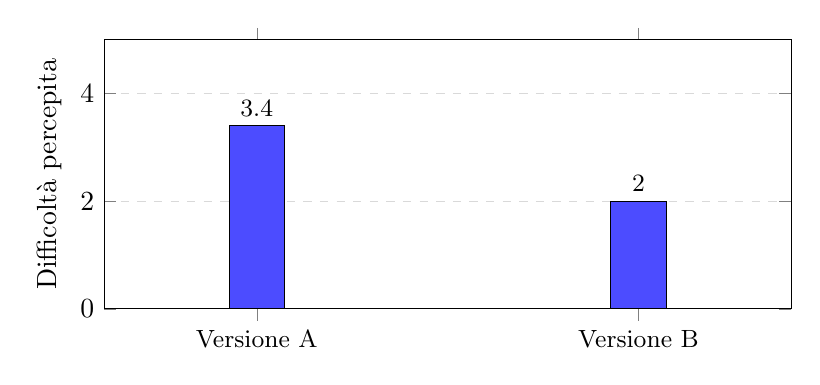
\begin{tikzpicture}
		\begin{axis}[
				ybar,
				bar width=20pt,
				width=0.85\textwidth,
				height=5cm,
				symbolic x coords={Versione A, Versione B},
				xtick=data,
				x tick label style={font=\small},
				ylabel={Difficoltà percepita},
				ymin=0, ymax=5,
				ymajorgrids=true,
				grid style={dashed, gray!30},
				enlarge x limits=0.4,
				nodes near coords,
				every node near coord/.style={font=\small, color=black},
			]
			\addplot+[
				ybar,
				fill=blue!70,
				draw=black
			] coordinates {
					(Versione A,3.40)
					(Versione B,2.00)
				};
		\end{axis}
	\end{tikzpicture}
	\caption{Confronto della difficoltà percepita tra Versione A e Versione B per S2.}
	\label{fig:6-s2-1}
\end{figure}

\begin{table}[H]
	\centering
	\footnotesize
	\renewcommand{\arraystretch}{1.2}
	\caption{Metriche prestazionali globali aggregate per lo Scenario S2.}
	\label{tab:6-s2-1}
	\begin{tabular}{|>{\raggedright\arraybackslash}p{2.2cm}|>{\centering\arraybackslash}p{1.5cm}|>{\centering\arraybackslash}p{1.5cm}|>{\centering\arraybackslash}p{1.5cm}|>{\centering\arraybackslash}p{1.5cm}|>{\centering\arraybackslash}p{1.8cm}|>{\centering\arraybackslash}p{1.6cm}|}
		\hline
		\rowcolor{gray!30}
		\textbf{S2}           & \multicolumn{2}{c|}{\textbf{Versione A}} & \multicolumn{2}{c|}{\textbf{Versione B}} & \textbf{Variazione \%} & \textbf{Rilevanza}                                            \\ \hline
		\textit{Success Rate} & \multicolumn{2}{c|}{100,00\%}            & \multicolumn{2}{c|}{100,00\%}            & \textbf{Invariato}     &                                                               \\ \hline
		\rowcolor{gray!30}
		                      & \textbf{Media}                           & \textbf{DEV.ST}                          & \textbf{Media}         & \textbf{DEV.ST}    & \multicolumn{2}{c|}{}                    \\ \hline
		\textit{Errori}       & 2,80                                     & 2,33605                                  & 0,467                  & 0,63994            & \textbf{-83,33\%}     & \pvalue{0,00104} \\ \hline
		\textit{Tempo}        & 4.37.16                                  & 0,10212                                  & 2.47.08                & 0,05400            & \textbf{-39,72\%}     & \pvalue{0,00382} \\ \hline
		\textit{Click}        & 50,60                                    & 18,34510                                 & 20,47                  & 6,06944            & \textbf{-59,55\%}     & \pvalue{0,00002} \\ \hline
		\rowcolor{gray!30}
		                      & \multicolumn{2}{c|}{\textbf{Mediana}}    & \multicolumn{2}{c|}{\textbf{Mediana}}    & \multicolumn{2}{c|}{}                                                                  \\ \hline
		\textit{Difficoltà}   & \multicolumn{2}{c|}{3}                   & \multicolumn{2}{c|}{2}                   & \multicolumn{2}{c|}{}                                                                  \\ \hline
	\end{tabular}
\end{table}

Il drastico calo degli errori e la considerevole riduzione dei click medi confermano l'efficacia della riprogettazione, evidenziando un flusso di lavoro semplificato che permette agli utenti di organizzare e caricare i materiali in modo assai più diretto.

\paragraph{Analisi qualitativa: commenti e osservazioni degli utenti}

Le osservazioni raccolte durante i test aiutano a spiegare le differenze emerse tra le due versioni. Nella versione originale (A), gli utenti hanno incontrato diverse difficoltà durante il caricamento e la gestione dei materiali.

\begin{itemize}
	\item \textbf{Flusso poco flessibile}: diversi partecipanti hanno espresso insoddisfazione per alcuni passaggi obbligati. In particolare, alcuni utenti hanno affermato che avrebbero ``preferito caricare direttamente il file creando la cartella nel mentre'', segnalando una procedura percepita come troppo rigida.
	\item \textbf{Difficoltà nel trovare le funzionalità AI}: alcuni utenti hanno tentato di caricare direttamente i file audio all'interno delle cartelle senza individuare facilmente gli strumenti di Intelligenza Artificiale dedicati alla trascrizione.

	\item \textbf{Feedback poco chiari}: il sistema non forniva indicazioni sufficienti quando alcuni campi obbligatori non venivano compilati. Di conseguenza, gli utenti non comprendevano immediatamente il motivo del mancato completamento dell'operazione. Ulteriore confusione è stata causata da alcuni valori preimpostati e da aggiornamenti improvvisi della pagina durante l'inserimento dei dati.
\end{itemize}

Per la versione post-riprogettazione (B), i commenti raccolti confermano invece un netto miglioramento dell'esperienza d'uso. La riduzione di click ed errori suggerisce che la riorganizzazione dei comandi, l'introduzione di feedback più chiari e il miglioramento del processo di caricamento abbiano reso il flusso più lineare. Diversi utenti hanno infatti definito la nuova procedura come ``intuitiva''.

\paragraph{Valutazione dell'effetto di apprendimento}

Analizzando i dati in base all'ordine di esecuzione (Tabella~\ref{tab:6-s2-2}), emerge come una struttura più chiara dell'interfaccia favorisca l'apprendimento delle attività richieste.

Nel gruppo che ha affrontato il test nella sequenza A--B, l'interazione iniziale con la versione originale ha fatto registrare un tempo medio di esecuzione pari a 5.44.07. Il successivo passaggio alla versione B ha prodotto un miglioramento solido ed empiricamente fondato, con il tempo medio che scende del 49,05\% per attestarsi a 2.55.20. Questo progresso trova piena conferma in diminuzioni altrettanto sistematiche e non attribuibili al caso per quanto riguarda sia la media degli errori (-81,82\%, da 3,67 a 0,67) sia quella dei click (-59,27\%, da 54,56 a 22,22).

Nel gruppo caratterizzato dall'ordine B--A, il tempo medio di esecuzione mostra un incremento nel passaggio dalla versione riprogettata a quella originale (da 2.34.50 a 2.57.00): questa variazione è tuttavia da interpretare come semplice trend descrittivo, non risultando statisticamente discriminante. Al contrario, si registrano decisi peggioramenti per le altre metriche operative nel passaggio alla versione A, confermati da forti riscontri nei test inferenziali. In particolare, la media degli errori aumenta significativamente dell'800,00\% (passando da 0,17 a 1,50) e il numero medio di click cresce del 150,47\% (da 17,83 a 44,67).

Tale quadro evidenzia come l'apprendimento non riesca a compensare i limiti strutturali della versione originale: pur avendo acquisito familiarità con il flusso di lavoro grazie all'esperienza positiva con la versione B, gli utenti hanno comunque riscontrato un incremento sistematico di errori e azioni necessarie per concludere il compito nell'interfaccia A.

\begin{table}[H]
	\centering
	\footnotesize
	\renewcommand{\arraystretch}{1.2}
	\caption{Confronto delle metriche prestazionali in funzione dell'ordine di esecuzione per lo Scenario S2.}
	\label{tab:6-s2-2}
	\begin{tabular}{|>{\raggedright\arraybackslash}p{2.2cm}|>{\centering\arraybackslash}p{1.0cm}|>{\centering\arraybackslash}p{1.0cm}|>{\centering\arraybackslash}p{1.8cm}|>{\centering\arraybackslash}p{1.6cm}|>{\centering\arraybackslash}p{1.0cm}|>{\centering\arraybackslash}p{1.0cm}|>{\centering\arraybackslash}p{1.8cm}|>{\centering\arraybackslash}p{1.6cm}|}
		\hline
		\rowcolor{gray!30}
		\textbf{Metrica}              & \multicolumn{4}{c|}{\textbf{Ordine A--B}}                                                 & \multicolumn{4}{c|}{\textbf{Ordine B--A}}                                                 \\ \cline{2-9} 
		\rowcolor{gray!30}
		                              & \textbf{A}          & \textbf{B}          & \textbf{Variazione \%} & \textbf{Rilevanza}        & \textbf{B}          & \textbf{A}          & \textbf{Variazione \%} & \textbf{Rilevanza}        \\ \hline
		\textit{Tempo (Media)}        & 5.44.07             & 2.55.20             & \textbf{-49,05\%}      & \pvalue{0,01267}          & 2.34.50             & 2.57.00             & \textbf{14,32\%}       & \pvalue{0,32504}          \\ \hline
		\textit{Errori (Media)}       & 3,67                & 0,667               & \textbf{-81,82\%}      & \pvalue{0,01200}          & 0,167               & 1,50                & \textbf{800,00\%}      & \pvalue{0,00146}          \\ \hline
		\textit{Click (Media)}        & 54,56               & 22,22               & \textbf{-59,27\%}      & \pvalue{0,00432}          & 17,83               & 44,67               & \textbf{150,47\%}      & \pvalue{0,00113}          \\ \hline
		\textit{Difficoltà (Mediana)} & 3                   & 2                   &                        & \pvalue{}                 & 2                   & 4                   &                        & \pvalue{}                 \\ \hline
	\end{tabular}
\end{table}

Le valutazioni di difficoltà percepita confermano questo andamento. Esaminando le risposte tramite la mediana, la versione B dimostra una stabilità eccellente con un valore pari a 2 in entrambi i gruppi, indicando come il nuovo flusso per la gestione di cartelle e funzionalità IA sia compreso agevolmente da tutti. Al contrario, la valutazione mediana della versione originale (A) si attesta a 3 per il gruppo A--B e sale a 4 per il gruppo B--A. Questa differenza trova perfetto riscontro qualitativo nei punteggi medi illustrati in Figura~\ref{fig:6-s2-2} (3,00 per A--B e 4,00 per B--A). L'aumento della difficoltà percepita per la versione A nel gruppo B--A suggerisce che l'esperienza diretta con un'interfaccia fluida e pulita renda gli utenti molto più critici verso le carenze del sistema originale, rendendo i blocchi e la scarsa intuitività della versione A ancora meno tollerabili anche a fronte di una conoscenza pregressa del compito.

\begin{figure}[H]
	\centering
	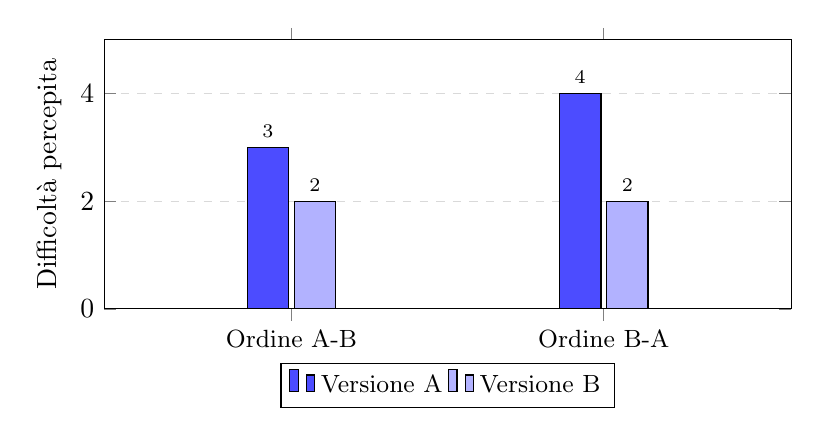
\begin{tikzpicture}
		\begin{axis}[
				ybar,
				bar width=15pt,
				width=0.85\textwidth,
				height=5cm,
				symbolic x coords={Ordine A-B, Ordine B-A},
				xtick=data,
				x tick label style={font=\small},
				ylabel={Difficoltà percepita},
				ymin=0, ymax=5,
				ymajorgrids=true,
				grid style={dashed, gray!30},
				enlarge x limits=0.6,
				legend style={at={(0.5,-0.2)}, anchor=north, legend columns=-1, font=\small},
				nodes near coords,
				every node near coord/.append style={font=\scriptsize, color=black},
			]
			\addplot+[
				fill=blue!70,
				draw=black
			] coordinates {
					(Ordine A-B,3.00)
					(Ordine B-A,4.00)
				};
			\addplot+[
				fill=blue!30,
				draw=black
			] coordinates {
					(Ordine A-B,2.00)
					(Ordine B-A,2.00)
				};
			\legend{Versione A, Versione B}
		\end{axis}
	\end{tikzpicture}
	\caption{Confronto della difficoltà percepita tra Versione A e Versione B per S2 in base all'ordine di esecuzione.}
	\label{fig:6-s2-2}
\end{figure}
